%--------------------------------------------------------------------------------------------------------------------------------------------VPN
\section{Virtual Private Networks }
Una rete privata virtuale consiste in una rete il cui accesso è regolamentato, che si appoggia a un protocollo di trasporto pubblico e condiviso, e che consente di garantire confidenzialità della comunicazione, accesso solo previa autenticazione, integrità dei dati e protezione da alcuni tipi di attacchi, ad esempio Man-in-the-middle o attacco replay.

\subsection{Architetture disponibili}
Una rete VPN può realizzare diversi tipi di collegamenti, per soddisfare esigenze diverse. Nei paragrafi successivi, si andranno ad analizzare i 3 tipi di architetture più comuni:
\begin{itemize}
    \item Gateway-to-Gateway
    \item Host-to-Host
    \item Host-to-Gateway
\end{itemize}

\subsubsection{Gateway-to-Gateway}
Consiste in una VPN che connette in maniera stabile due reti. Questa configurazione permette ad esempio di estendere una rete privata tra diverse location geograficamente separati e distanti a piacere, oppure di garantire a una serie di uffici un accesso sicuro a un data center.

\subsubsection{Host-to-Host}
Questa configurazione è la meno comune. Consiste nello stabilire una comunicazione diretta tra due host, in cui uno fa da server VPN e l'altro da client VPN. Un caso d'uso potrebbe essere un amministratore di sistema che deve fare gestione remota di un apparecchio.

\subsubsection{Host-to-Gateway}
In questa modalità, il risultato che si ottiene è lo stesso che si avrebbe connettendo un host alla rete locale in cui risiede il server VPN.
È usata principalmente per offrire un accesso sicuro da remoto alla rete. Quando l'host vuole instaurare una connessione VPN con il server, gli viene richiesto di autenticarsi.

\subsection{Perché soddisfano i requisiti}
Una VPN in configurazione Host-to-Gateway si prospetta come la soluzione più pratica e funzionale per soddisfare le necessità dell'azienda e dei suoi dipendenti, garantendo loro la possibilità di accedere alle risorse interne attraverso un canale di comunicazione privato, ad accesso controllato, criptato e dove è assicurata l'integrità dei dati.

\subsection{Soluzioni principali}
Tra le soluzioni VPN più comuni troviamo:
\begin{itemize}
    \item Point-to-Point Tunneling Protocol
    \item Internet Protocol Security
    \item OpenVPN
    \item Wireguard
    \item Mettere Esempio di Web Based SSL VPN %https://www.firewall.cx/cisco-technical-knowledgebase/cisco-services-tech/342-cisco-web-vpn.html
\end{itemize}

%---------------------------------------------------------------------------------------------------------------------------------------------IPSec
% BUONO https://pctempo.com/openvpn-vs-ikev2-vs-pptp-vs-l2tp-ipsec-vs-sstp/

% https://it.wikipedia.org/wiki/IPsec https://github.com/sunknudsen/privacy-guides/blob/master/how-to-self-host-hardened-strongswan-ikev2-ipsec-vpn-server-for-ios-and-macos/README.md 

% 1.	Come è nato
% 2.	Tipo incapsulamento
% 3.	Overhead - byte sprecati per pacchetto
% 4.	Livello a cui lavora
% 5.	Protocolli usati
% 6.	Cifratura usata ? hw o sw, limitata se non aggiorni hw ma più veloce, e il contrario

\section{Internet Protocol Security}
\subsection{Panoramica}
IP Security è una suite di protocolli il cui obiettivo è rendere sicura la comunicazione tra due computer attraverso una rete IP.
Contiene protocolli per la mutua autenticazione degli host e per la negoziazione delle chiavi di cifratura da usare durante la sessione.
In molti contesti, rendere sicuro il livello di rete (L3 OSI) è una soluzione migliore rispetto a rendere sicuro il livello di trasporto (L4 OSI) o di presentazione (L7 OSI), in quanto offre un ulteriore punto di controllo per gli amministratori e più flessibilità nell'analizzare, e gestire, ogni singolo pacchetto IP.
IPSec supporta l'autenticazione a livello di rete, autenticazione del mittente, integrità dei dati, cifratura, e protezione dagli attacchi replay, protezione dall'analisi del traffico e controllo degli accessi.

\subsection{Transport mode vs Tunnel mode}
The IPsec protocols AH and ESP can be implemented in a host-to-host transport mode, as well as in a network tunneling mode.

\begin{figure}[ht]
    \centering
    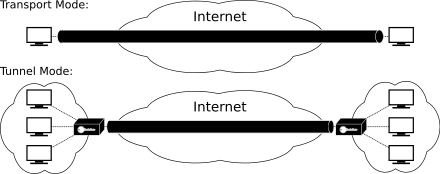
\includegraphics[width=8cm]{figure/ipsec_modes.png}
    \caption{Transport mode vs Tunnel mode diagram}
\end{figure}


\subsubsection{Transport mode}
In transport mode, generalmente solo il payload del pacchetto IP è cifrato o autenticato. L'indirizzamento non cambia, dato che l'header IP non è né modificato né cifrato; tuttavia, quanto si usa il protocollo Authentication Header - approfondito in seguito - l'indirizzo IP non può essere modificato da Network Address Translation, in quanto una modifica al campo invaliderebbe l'hash. Il livello di trasporto e di applicazione sono sempre certificati da un hash, quindi il loro contenuto non può essere modificato in alcun modo, ad esempio utilizzando una traduzione dei numeri delle porte.
Un superamento delle problematiche causate dall'attraversamento di NAT è definito dalle RFC che descrivono il meccanismo NAT-T, ma che va oltre gli scopi di questa tesi.

\subsubsection{Tunnel mode}
In tunnel mode, l'intero pacchetto è cifrato e autenticato. È dunque incapsulato all'interno di un nuovo pacchetto IP con un nuovo header IP.
Generando un nuovo header IP, non si incontra nessuna difficoltà nell'attraversamento di NAT.


\subsection{Protocolli utilizzati}
IPSec utilizza i seguenti protocolli per stabilire una connessione sicura. Sia AH che ESP, descritti in seguito, possono lavorare in tunnel mode o in transport mode.

\subsubsection{Authentication Header}
\begin{figure}[ht]
    \centering
    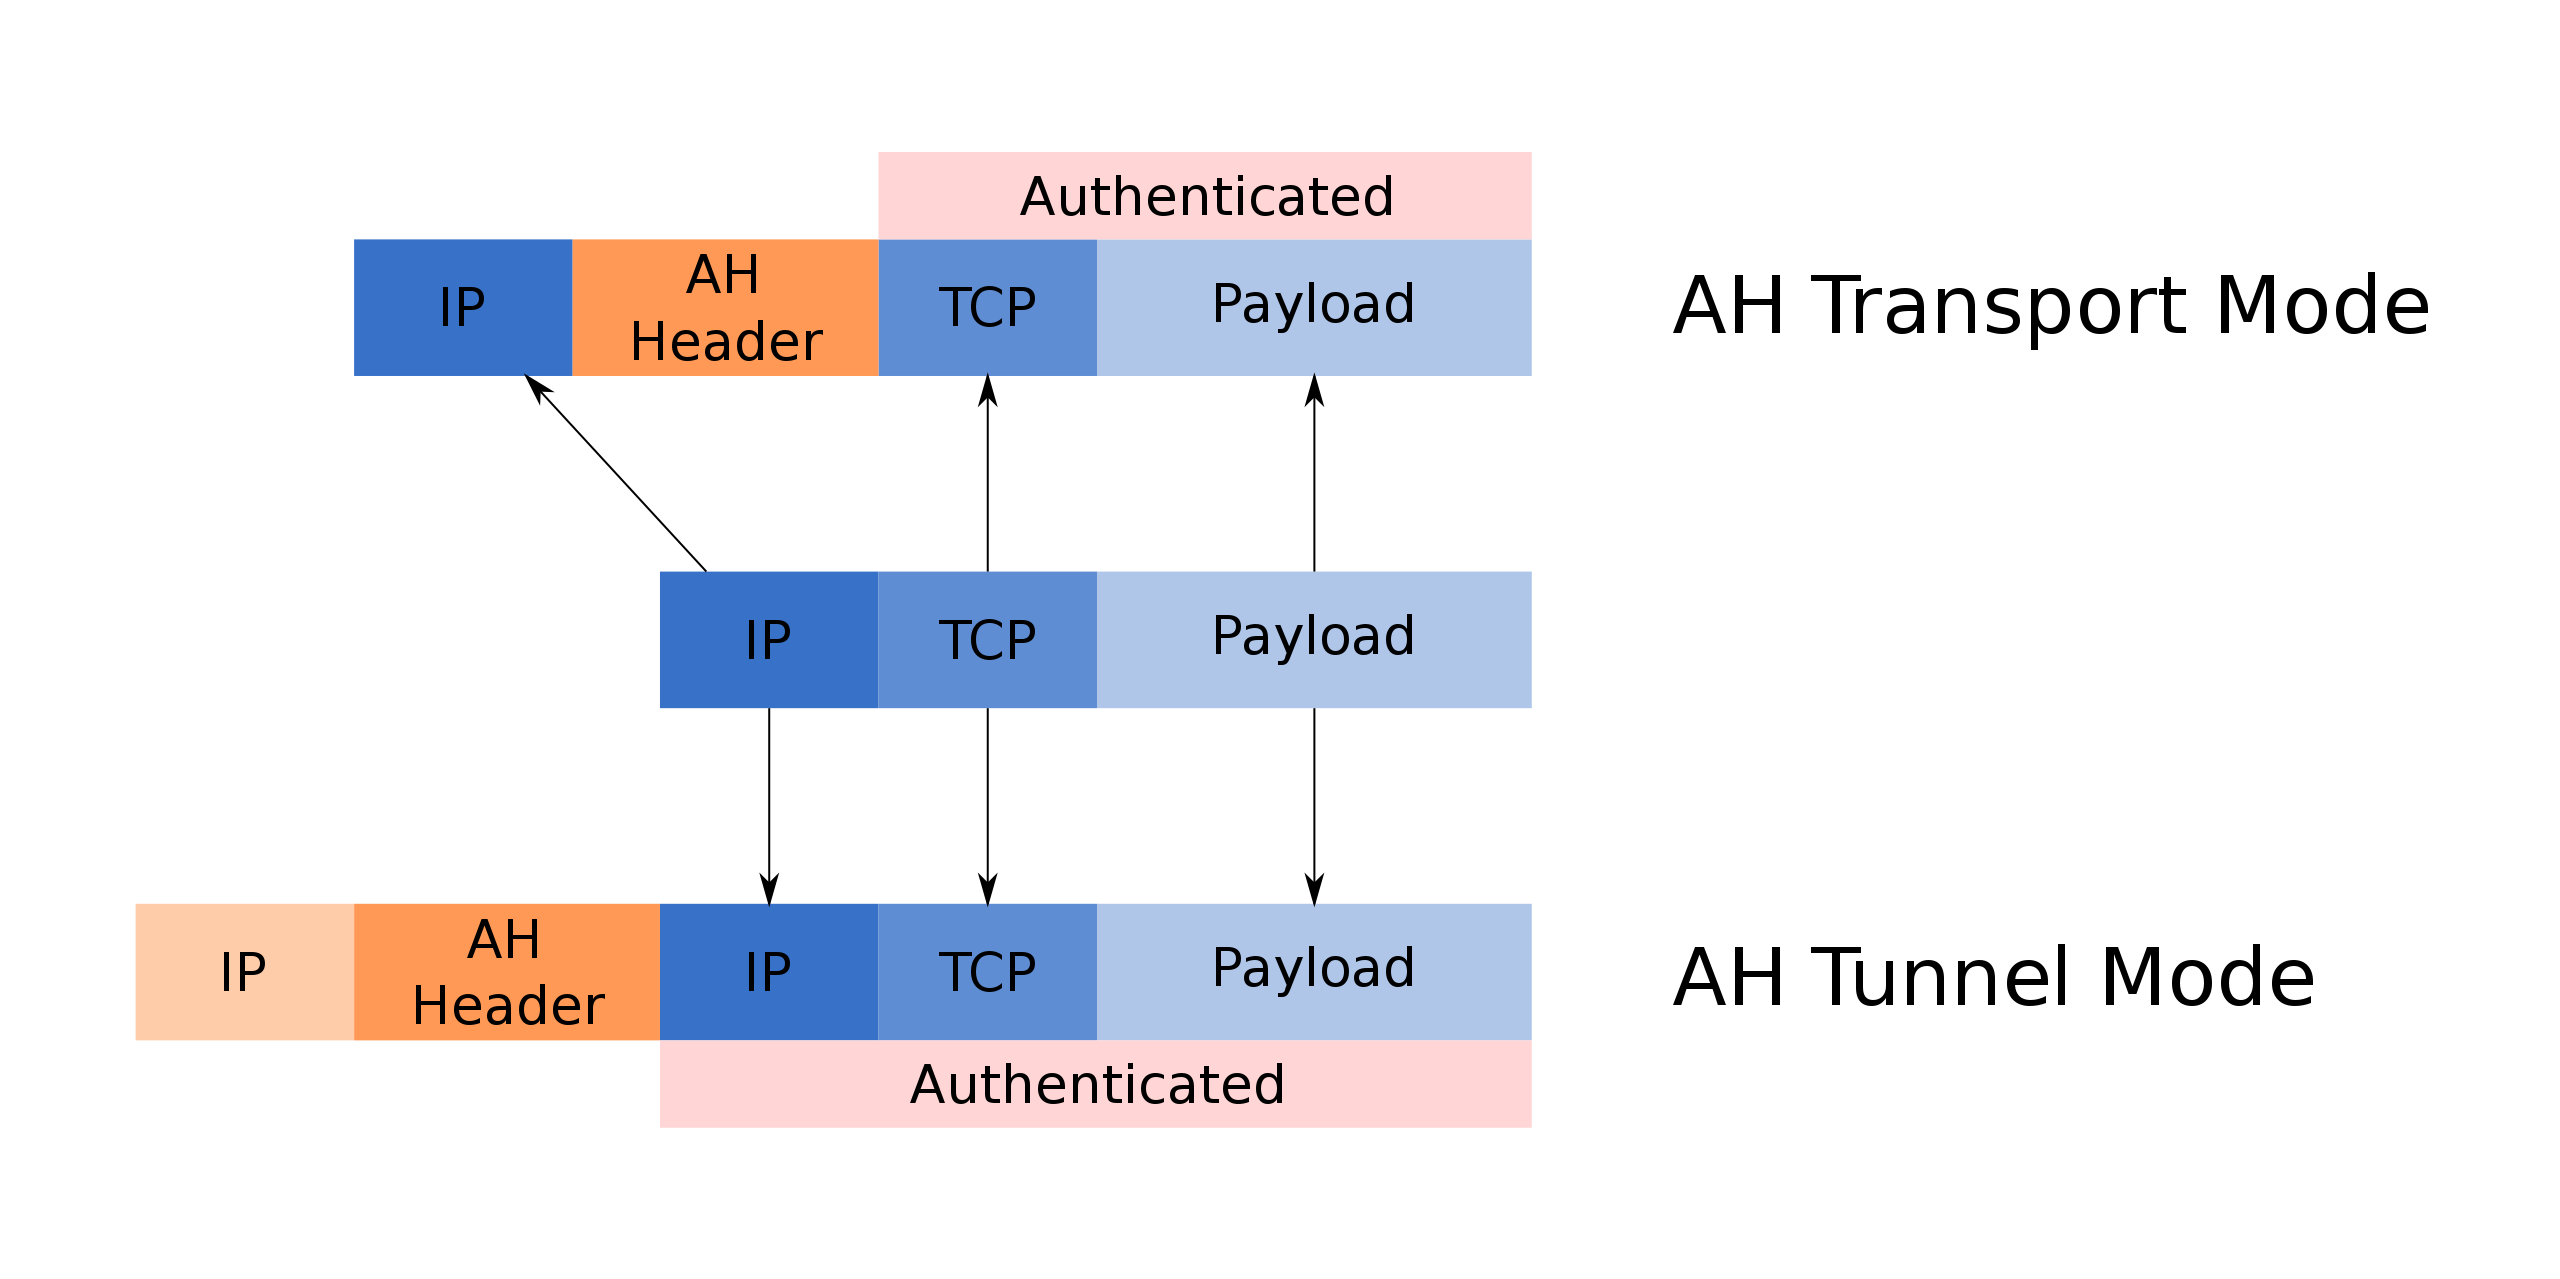
\includegraphics[width=10cm]{figure/ah_tun_trasp.png}
    \caption{Authentication Header packet formats}
\end{figure}

Authentication Header \cite[RFC4302]{RFC4302} garantisce integrità per tutti gli header dei pacchetti, ad eccezione di alcuni campi dell'header IP, e autenticazione del mittente. Se configurato, è anche possibile utilizzarlo per offrire protezione dagli attacchi replay. AH si interfaccia direttamente con IP, utilizzamndo il protocollo IP numero 51.
AH autentica l'intero datagramma, ad eccezione dei campi variabili. Tuttavia, le informazioni contenute nel datagramma sono trasferite in chiaro e, dunque, leggibili da uno sniffer. Per questo motivo, AH non soddisfa i requisiti di sicurezza richiesti.

\subsubsection{Encapsulating Security Payload}
\begin{figure}[ht]
    \centering
    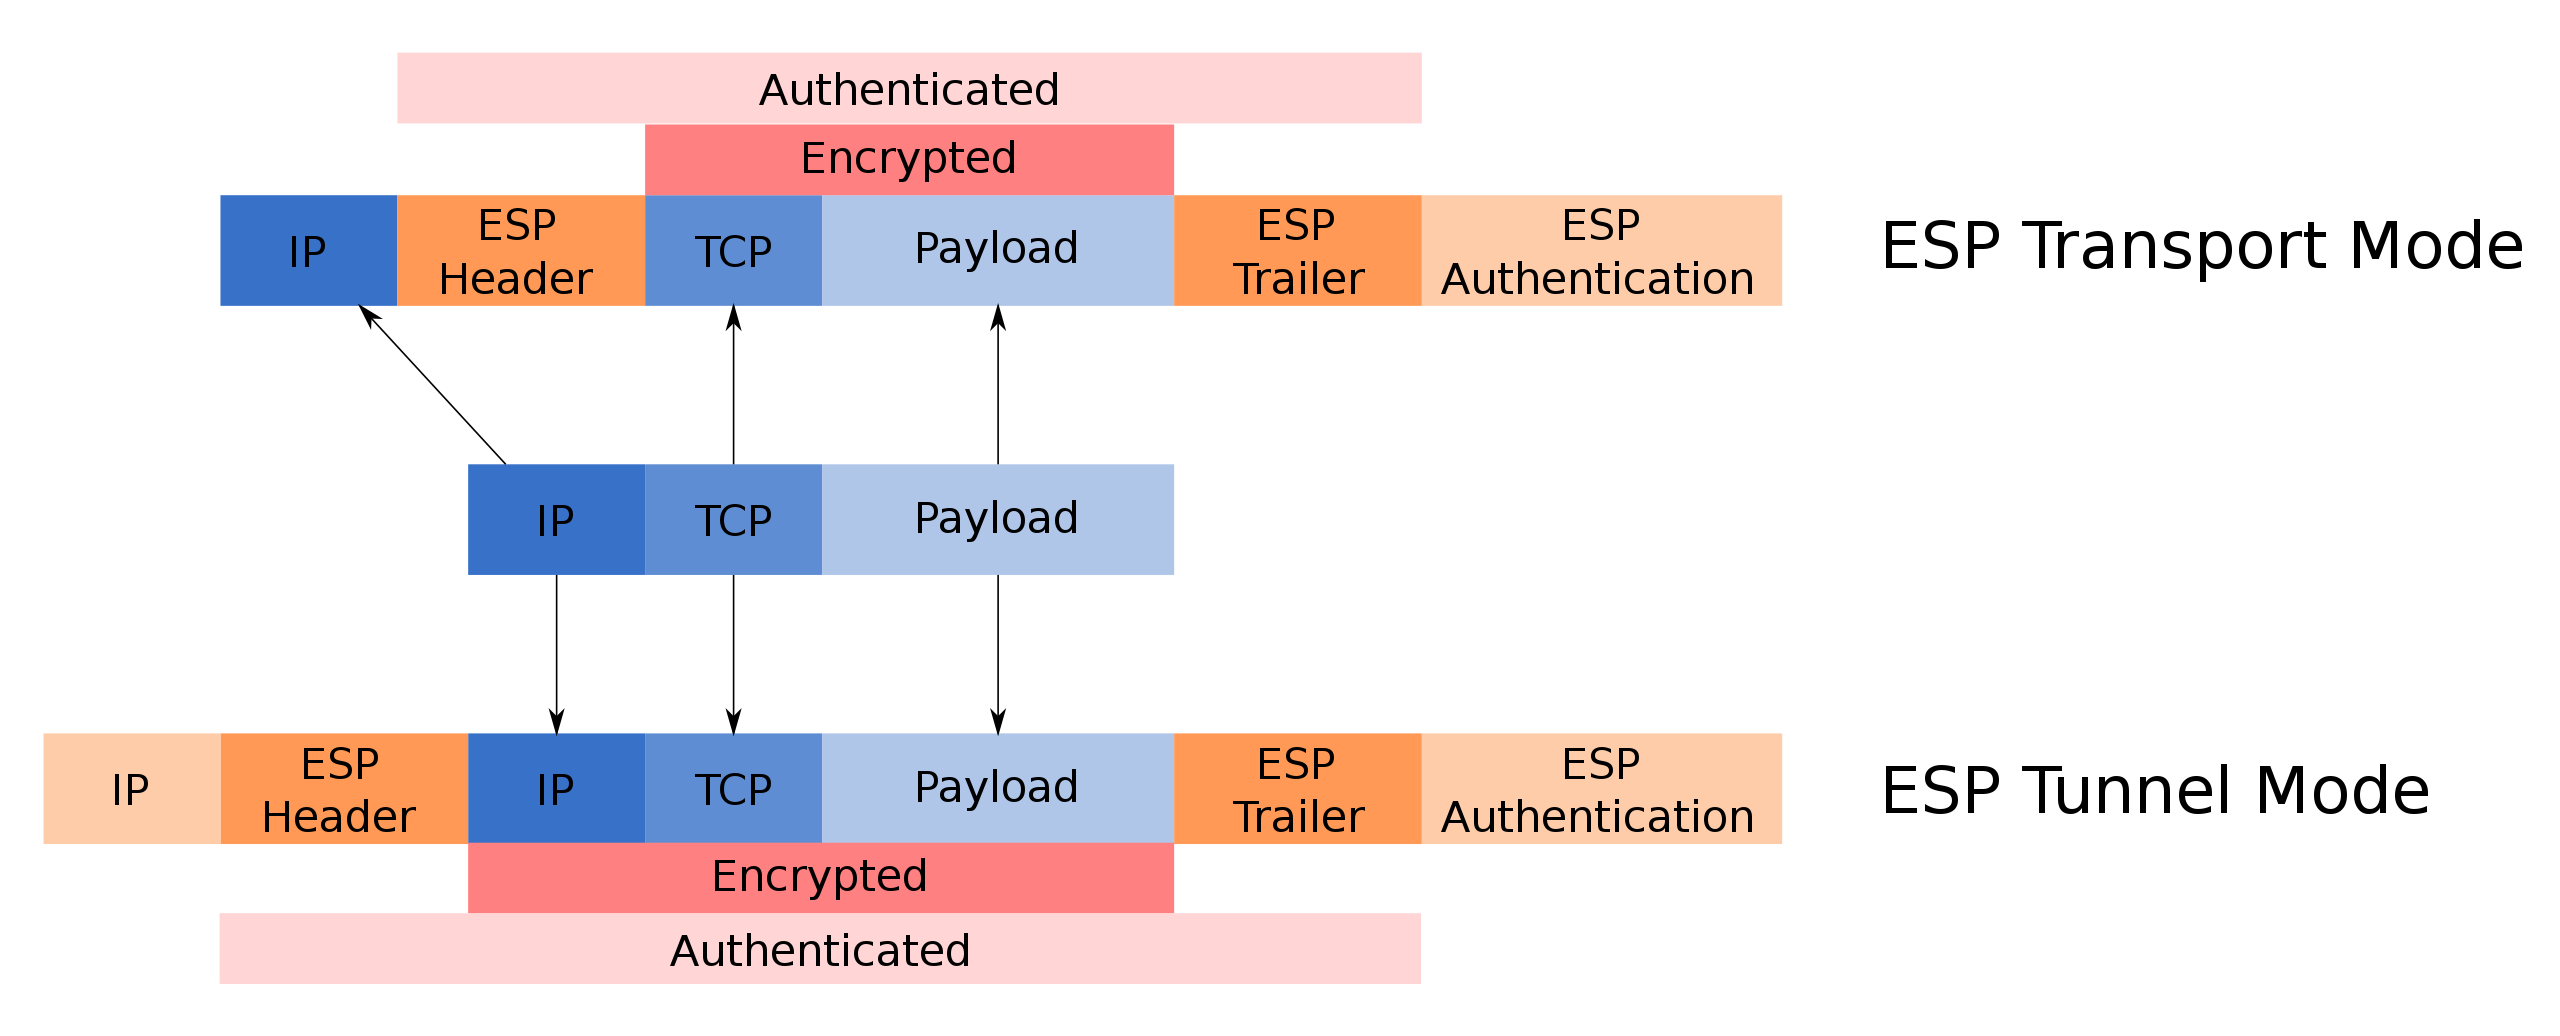
\includegraphics[width=10cm]{figure/esp_tun_trasp.png}
    \caption{Encapsulating Security Payload packet formats}
\end{figure}
Encapsulating Security Payload \cite[RFC4303]{RFC4303} offre confidenzialità dei fati, autenticazione del mittente, controllo di integrità e protezione da attacchi relay.
In Transport mode, non autentica né cifra l'header IP: cioè potrebbe esporre le informazioni contenute a potenziali attacchi mentre il pacchetto è in transito.
Tuttavia, la Transport mode necessita di meno potenza computazionale, ottenendo un overhead minore della tunnel mode, rinunciando a una maggior sicurezza.

In Tunnel mode, viene creato un nuovo header IP e usato come header esterno del pacchetto, eguito dall'header ESP e poi il pacchetto originale (sia header IP che payload originale).
L'ESP Trailer e gli opzionali dati di autenticazione sono aggiunti dopo il payload.
Quando si usano cifratura e autenticazione contemporaneamente, ESP protegge completamente il pacchetto orginale, perché diventa il payload del nuovo pacchetto ESP.
Da notare è che non viene protetto il nuovo header IP.
Un gateway deve necessariamente usare ESP in Tunnel mode.

\subsubsection{Internet Key Exchange v2}
Ancora del testo---IKE è un acronimo per Internet key exchange ed è il protocollo usato per stabilire una security association nella suite di protocolli IPsec. Questo protocollo è definito in RFC 4306.  ---

Internet Key Exchange \cite[RFC4306]{RFC4306} è un protocollo che svolge la funzione di negoziazione, gestione e creazione delle Security Associations. Una SA è un insieme di regole necessarie a definire le funzionalità e i sistemi di sicurezza per stabilire una connessione IPSec. Può essere definita manualmente, anche se non scala dovutamente con VPN di grandi dimensioni. Un metodo più comune è quello di usare una delle cinque possibili modalità di scambio: main, aggressive, quick, informational e group.
Le modalità sono differenti per velocità e l'uso di funzioni di cifratura. IKEv2 è la versione più recende di IKE e migliora il protocollo rendendolo più sempice, garantendo affidabilità nel recapito dei messaggi, protezione contro attacchi di tipo DenialOfService e migliora l'uso di IKE su gateways NAT.
È un protocollo di livello applicazione e utilizza il protocollo UDP come protocollo di trasporto; la porta su cui viene stabilita la connessione è 500.

\subsection{Cifratura}
IPSec supporta diversi protocolli di cifratura, tra cui AES, Blowfish, Triple DES, ChaCha e DES-CBC. Inoltre, usa due tipi di cifratura: simmetrica e asimmetrica. In una codifica simmetrica, una chiave è condivisa tra gli utenti, mentre una asimmetrica fa affidamento su entrambe le chiavi pubbliche e private. La codifica asimmetrica è considerata più sicura: molti utenti condividono la chiave pubblica, ma la sicurezza fa affidamento sulla chiave privata - protetta a tutti costi - che non ha bisogno di essere condivisa con nessuno (a differenza di una chiave simmetrica).
IPSec usa la cifratura asimmetrica per instaurare una connessione sicura, per poi sfruttare quella simmetrica per migliorare la velocità di collegamento. Per quello che riguarda il collegamento, è compatibile sia con UDP che con TCP.


\subsection{Autenticazione}
L'autenticazione a chiave pubblica e privata assicura che mittenti e destinatari stiano effettivamente comunicando con il giusto partner. IPSec support molteplici sistemi di autenticazione, tra cui: HMAC-SHA1/SHA2, certificate authorities (CAs), RSA, ECDSA, e pre-shared key (PSK). Ogni tipologia ha i suoi pregi e difetti e casi d'uso in cui è preferibile. Ogni protocollo punta a garantire che i dati rimangano sicuri e affidabili attraverso il loro tragitto.

\subsection{Implementazioni}
StrongSwan è una implementazione open-source di IPSec per Linux. Supporta funzionalità come IPv6, certificati X.509 a chiave pubblica, liste di certificati revocati, storage di chiavi RSA private su smartcard e implementazione completa del protocollo IKEv2.re.

\subsection{Considerazioni}
Ancora del testo
%---------------------------------------------------------------------------------------------------------------------------------------------PPTP
% https://www.ivpn.net/pptp-vs-ipsec-ikev2-vs-openvpn-vs-wireguard/

\section{PPTP}
\subsection{Panoramica}
Si tratta di uno dei più vecchi protocolli VPN in uso ancora oggi, ma in quanto tale ha alcune gravi criticità date dall'età. Ad esempio, la crittografia a 128 bit e il protocollo usato per l'autenticazione (MS-CHAP) contenente note vulnerabilità lo rendono ormai un protocollo insicuro, da evitare se le informazioni che transitano sono sensibili.
Tuttavia, è estremamente semplice da configurare e il più veloce dal punto di vista prestazionale, il che lo rende ideale per usi quali streaming video o l'utilizzo di VPN su terminali con potenze di calcolo estremamente limitate.
È stato sviluppato da Microsoft nel 1999 \cite[RFC2637]{RFC2637} e lavora instaurando un canale di controllo tra i due peers sulla porta 1723 TCP e un tunnel GRE su cui transitano effettivamente i dati.

\subsection{Protocolli utilizzati}
\subsubsection{Generic Routing Encapsulation}
GRE è un protocollo di tunneling sviluppato da Cisco Systems che può incapsulare un'ampia varietà di protocolli di livello di rete all'interno di collegamenti Point-to-Point o Point-to-Multipoint virtuali su una rete IP.

\subsection{Cifratura}
PPTP non specifica nessuna

\subsection{Autenticazione}
Ancora del testo

\subsection{Considerazioni}
Ancora del testo

%----------------------------------------------------------------------------------------------------------------------------------------------OpenVPN
% https://en.wikipedia.org/wiki/OpenVPN 
\section{OpenVPN}
\subsection{Panoramica}
OpenVPN è una VPN SSL che permette di incanalare tutto il traffico di una sottorete attraverso una unica porta UDP o TCP, e fa affidamento su OpenSSL. Come le altre soluzioni VPN, OpenVPN servizi essenziali di sicurezza quali autenticazione, cifratura, integrità dei dati e controllo degli accessi.
Supporta due modalità di lavoro, routing e bridging:
\begin{itemize}
    \item[Routing] consiste nell'interconnessione di due sottoreti indipendenti, dove il server VPN (generalmente installato sul router) inoltra i pacchetti all'indirizzo IP specificato in fase di configurazione. Si tratta quindi di un collegamento a livello 3 del modello OSI.
    \item[Bridging] è una modalità che lavora esclusivamente all'interno di una sottorete; il funzionamento è analogo a quello di uno switch ethernet fisico.
\end{itemize}

OpenVPN è una soluzione che lavora in user space, dunque l'overhead generato è maggiore in quanto sono necessarie molteplici copie dei pacchetti affiché siano trasferiti dal kernel space allo user space. Supporta l'intero insieme delle funzionalità di TLS, necessitando di una ampia code base, mostrando un maggior potenziale a soffrire di vulnerabilità.

\subsection{Protocolli utilizzati}
Come precedentemente acccennato, OpenVPN usa la libreria di OpenSSL, che implementa il protocollo Transport Layer Security, progettato per offrire una connessione sicura attraverso una rete non sicura.
A differenza del puro TLS, OpenVPN offre all'utente la possibilità di utilizzare una pre-shared key per generare quel che è noto come HMAC firewall, che autentica tutta la sequenza di handshake TLS.

Essendo UDP un protocolllo non connesso, i pacchetti IP criptati e firmati che sono incanalati tramite UDP, non hanno nessuna garanzia di affidabilità. L'affidabilità necessaria per una sicura autenticazione è garantita, però, dal protocollo TLS che utlizza TCP come protocollo di trasporto.
È importante notare che il canale dati e il canale di controllo transitano all'interno dello stesso tunnel UDP (o TCP). L'incapsulamento dei pacchetti è descritto dal seguente diagramma.

\begin{figure}
    \centering
    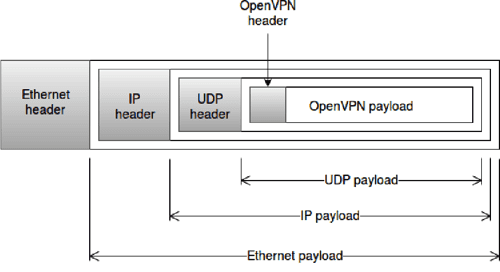
\includegraphics[width=8cm]{figure/OVPN_packet.png}
    \caption{Dettaglio di un pacchetto OpenVPN}
\end{figure}

La struttura mostrata si applica a tutti i pacchetti OpenVPN; tuttavia, differenti pacchetti avranno differenti payloads.


\subsubsection{Secure Socket Layer/Transport Layer Security VPNs}
Il protocollo Transport Layes Security, originariamente noto come Secure Socket Layer, è un protocollo progettato per garantire una connessione sicura attraverso una rete non sicura. TLS permette autenticazione di client e server, integrità dei dati e confidenzialità. Per l'autenticazione usa i certificati X.509 \cite[RFC5280]{RFC5280} con una crittografia asimmetrica e si occupa di negoziare una chiave di sessione simmetrica.
Un vantaggio delle VPN SSL rispetto a quelle basate su IPSec è che riescono a lavorare anche in reti protette da firewall molto stringenti, in quanto la maggior parte delle aziende non filtra il traffico TCP sulla porta 443, essendo normalmente usato dai dipendenti per accedere a Internet. OpenVPN di default utilizza la porta 1194 UDP, ma, nel caso quella porta fosse chiusa, può utilizzare la 443 TCP.


\subsection{Tunnel TCP vs UDP}
Premesso che attraverso i tunnel VPN passa traffico sia TCP che UDP, anche i tunnel stessi possono essere realizzati con connessioni TCP o UDP.

Il protocollo TCP utilizza notevoli algoritmi per assicurare un recapito correto dei dati al destinatario. Avere due connessioni TCP una dentro l'altra forzera gli algoritmi di entrambe le connessioni a lavorare in parallelo. Non essendo TCP progettato per lavorare in quella condizione, si potrebbe andare incontro a problemi quali il \emph{retransmission problem}, \emph{TCP meltdown} e doppia ritrasmissione. Questi problemi potrebbero verificarsi nel momento in cui entrambe le connessioni stanno tentando di ritrasmettere pacchetti.

Tutto ciò non vale per il protocollo UDP, che come descritto precedentemente, è un protocollo non connesso senza nessuna garanzia che il messaggio raggiunga correttamente il destinatario. A discapito dell'affidabilità, si possono ottenere velocità di trasmissione notevolmente superiori.


\subsection{Cifratura}
Ancora del testo

\subsection{Autenticazione}
In contrast to pre-share static key mode, TLS mode uses TLS protocol to authenticate, establish secure channel and exchange the symmetric tunnel session key between peers.
Just like in pre-shared static key mode, session key is used to en- crypt the data tunnel, however, the authentication and symmetric key exchange take place using TLS protocol.
This not only provides an automatic and secure way of distributing symmetric keys, but also a way to renew the symmetric key at any point during the communication.
The aforementioned aspect of the TLS mode provides the Perfect Forward Secrecy, which is not present in pre-shared static key mode.
The structure of the tunnel session key derivation TLS packet, as shown in Wireshark, can be seen in Fig. 4.
The transfer of tunnel session keys are encrypted and carried inside the TLS Record layer, so it cannot be decrypted without the proper TLS certificates. The two main steps in this protocol are shown below.
1. Negotiation of the TLS connection. Both sides of the connection are au- thenticated by exchanging certificates and verifying the certificate of the opposing side. If the authentication is successful, the protocol proceeds wit the step two. Otherwise, the connection is terminated.
2. Tunnel session keys are negotiated over the already established secure TLS channel. The tunnel session key derivation TLS packet structure depends on the OpenVPN key method being used. TLS mode supports two key methods, which are described below.
If the first key method is used, then the tunnel session keys are derived from OpenSSL cryptographic library RAND bytes function.
The tunnel session key derivation TLS packet structure is shown in Tab. 3.
(b) If the second key method is used, (default in the OpenVPN 2.0+), then the tunnel session keys are derived from the RAND bytes func- tion passed through the TLS pseudo-random function (TLS PRF).
In order to successfully construct a OpenVPN client, it is important to un- derstand the key differences explained in this chapter between the TLS modes, key methods and their respective packet structures.

\subsection{Misure di sicurezza aggiuntive}
OpenVPN offre diverse funzionalità di sicurezza: cifratura fino a 256-bit attraverso la libreria OpenSSL, anziché supportare IKE; lavora in user space, senza quindi necessità di effettuare operazioni sullo stack IP, e quindi operazioni kernel; ha la possibilià di far cadere i privilegi di root; entrare in una \emph{chroot jail} dopo l'inizializzazione; applicare un SELinux context dopo l'inizializzazione; offre supporto alle smartcard attraverso i token basati su PKCS 11.

\subsection{Considerazioni}
Ancora del testo

%--------------------------------------------------------------------------------------------------------------------------------------------Wireguard
\section{WireGuard}
\subsection{Panoramica}
In Linux, the standard solution for encrypted tunnels is IPsec, which uses the Linux transform (“xfrm”) layer. Users fill in a kernel structure determining which ciphersuite and key, or other transforms such as compression, to use for which selector of packets traversing the subsystem. Generally a user space daemon is responsible for updating these data structures based on the results of a key exchange, generally done with IKEv2 [13], itself a complicated protocol with much choice and malleability. The complexity, as well as the sheer amount of code, of this solution is considerable. Administrators have a completely separate set of firewalling semantics and secure labeling for IPsec packets. While separating the key exchange layer from the transport encryption— or transformation—layer is a wise separation from a semantic viewpoint, and similarly while separating the transformation layer from the interface layer is correct from a networking viewpoint, this strictly correct layering approach increases complexity and makes correct implementation and deployment prohibitive.
WireGuard does away with these layering separations. Instead of the complexity of IPsec and the xfrm layers, WireGuard simply gives a virtual interface—wg0 for example—which can then be administered using the standard ip(8) and ifconfig(8) utilities. After configuring the interface with a private key (and optionally a pre-shared symmetric key as explained in section 5.2) and the various public keys of peers with whom it will communicate securely, the tunnel simply works. Key exchanges, connections, disconnections, reconnections, discovery, and so forth happen behind the scenes transparently and reliably, and the administrator does not need to worry about these details. In other words, from the perspective of administration, the WireGuard interface appears to be stateless. Firewall rules can then be configured using the ordinary infrastructure for firewalling interfaces, with the guarantee that packets coming from a WireGuard interface will be authenticated and encrypted. Simple and straightforward, WireGuard is much less prone to catastrophic failure and misconfiguration than IPsec. It is important to stress, however, that the layering of IPsec is correct and sound; everything is in the right place with IPsec, to academic perfection. But, as often happens with correctness of abstraction, there is a profound lack of usability, and a verifiably safe implementation is very difficult to achieve. WireGuard, in contrast, starts from the basis of flawed layering violations and then attempts to rectify the issues arising from this conflation using practical engineering solutions and cryptographic techniques that solve real world problems.

For key distribution, WireGuard draws inspiration from OpenSSH, for which common uses include a very simple approach toward key management. Through a diverse set of out-of-band mechanisms, two peers generally exchange their static public keys. Sometimes it is simple as PGP-signed email, and other times it is a complicated key distribution mechanism using LDAP and certificate authorities. Importantly, for the most part OpenSSH key distribution is entirely agnostic. WireGuard follows suit. Two WireGuard peers exchange their public keys through some unspecified mechanism, and afterward they are able to communicate. In other words, WireGuard's attitude toward key distribution is that this is the wrong layer to address that particular problem, and so the interface is simple enough that any key distribution solution can be used with it. As an additional advantage, public keys are only 32 bytes long and can be easily represented in Base64 encoding in 44 characters, which is useful for transferring keys through a variety of different mediums.
Finally, WireGuard is cryptographically opinionated. It intentionally lacks cipher and protocol agility. If holes are found in the underlying primitives, all endpoints will be required to update. As shown by the continuing torrent of SSL/TLS vulnerabilities, cipher agility increases complexity monumentally. WireGuard uses a variant of Trevor Perrin's Noise [23]—which during its development received quite a bit of input from the authors of this paper for the purposes of being used in WireGuard—for a 1-RTT key exchange, with Curve25519 [5] for ECDH, HKDF [15] for expansion of ECDH results, RFC7539 [17]'s construction of ChaCha20 [3] and Poly1305 [8] for authenticated encryption, and BLAKE2s [2] for hashing. It has built-in protection against denial of service attacks, using a new crypto-cookie mechanism for IP address attributability.
Similarly opinionated, WireGuard is layer 3-only; as explained below in section 2, this is the cleanest approach for ensuring authenticity and attributability of the packets. The autqwhors believe that layer 3 is the correct way for bridging multiple IP networks, and the imposition of this onto WireGuard allows for many simplifications,
3
resulting in a cleaner and more easily implemented protocol. It supports layer 3 for both IPv4 and IPv6, and can encapsulate v4-in-v6 as well as v6-in-v4.
WireGuard puts together these principles, focusing on simplicity and an auditable codebase, while still being extremely high-speed and suitable for a modicum of environments. By combining the key exchange and the layer 3 transport encryption into one mechanism and using a virtual interface rather than a transform layer, WireGuard indeed breaks traditional layering principles, in pursuit of a solid engineering solution that is both more practical and more secure. Along the way, it employs several novel cryptographic and systems solutions to achieve its goals.

\subsection{Protocolli utilizzati}
Ancora del testo

\subsubsection{Something}
Ancora del testo

\subsection{TCP vs UDP}
Ancora del testo

\subsection{Cifratura}
Ancora del testo

\subsection{Autenticazione}
Ancora del testo

\subsection{Considerazioni}
Ancora del testo